\begin{frame}[t]
    \frametitle{Working on paper: A Computer-Scientists view}

    Doing Theoretical Physics often requires lengthy analytical calculations
    \vspace{0.8em}

    \begin{columns}[t]
        \column{0.4\textwidth}
            \textbf{Advantages} of working on paper:
            \begin{itemize}
                \item No barrier to entry (required Skill \& technology)
                \item Maximum liberty how to operate
                \item Fast iteration for high variation workload
                \item "Offline" available
            \end{itemize}
        
        \column{0.4\textwidth}
            \textbf{Problems} of working on paper:
            \begin{itemize}
                \item Repetitive tasks not automizable
                \item Error-prone and time- consuming to fix mistakes
                \item Difficult \& non-standard to share/archive
                \item No version-control
                \item Need to produce final version anyway
            \end{itemize}
            
    \end{columns}
\end{frame}

\note[enumerate]{
    \item Comparison of advantages/disatvantages of doing calculations "by hand"
    \item Advantages
    \begin{itemize}
        \item No skills required to learn, writing is natural, every new symbol can just be written
        \item Operational Libery (cross out stuff as please, swap whatever without "proof")
        \item For completely different approaches no new tool is needed (lern that integral cannot be solved with a specific strategy that you tool doesn't support: out of luck)
        \item Hard to loose access to taken notes, produce them without internet/power
    \end{itemize}
    \item Disatvantages
    \begin{itemize}
        \item Many tasks are repetetive, trivial and unfunny to do, paper cannot automize
        \item Sign errores, copy errors happen too often
        \item Sharing and archiving is non-standart. Many standarts exist for e.g. sharing latex
        \item No version-control (git): hard for people that are used to it like me. Cannot just do stuff and later revert if it didn't work
        \item Need to write the pretty version in the computer anyway
    \end{itemize}
}

\begin{frame}
    \frametitle{Examples from "Theoretical Solid State Physics"}

    \hspace{-1cm}
    \makebox[\textwidth][c]{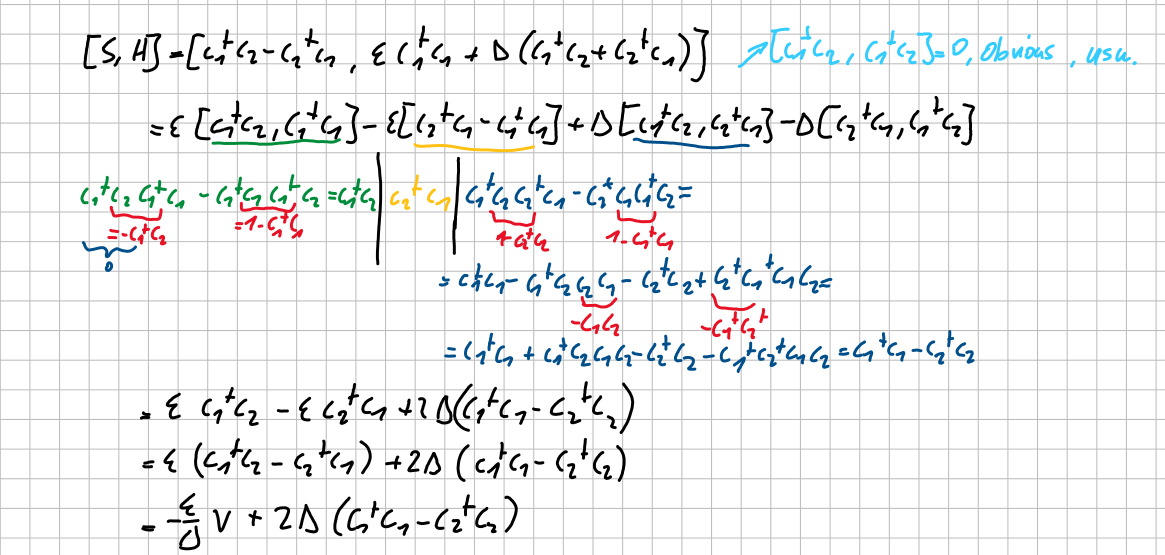
\includegraphics[width=0.85\textwidth]{math-manipulator-calculations/fkp_page_15.png}}
    
\end{frame}

\note[enumerate]{
    \item From the lecture "Theoretical Solid State Physics" (Theoretische Festkörperphysik), helt by Markus Heyl in WS 22/23
    \item Sheet 3, Problem 2: Schrieffer-Wolf transformation
    \item Rather simple calculation, still contains sing mistakes (that here luckily averaged out)
}

\begin{frame}
    \frametitle{Examples from "Theoretical Solid State Physics"}

    \hspace{-1cm}
    \makebox[\textwidth][c]{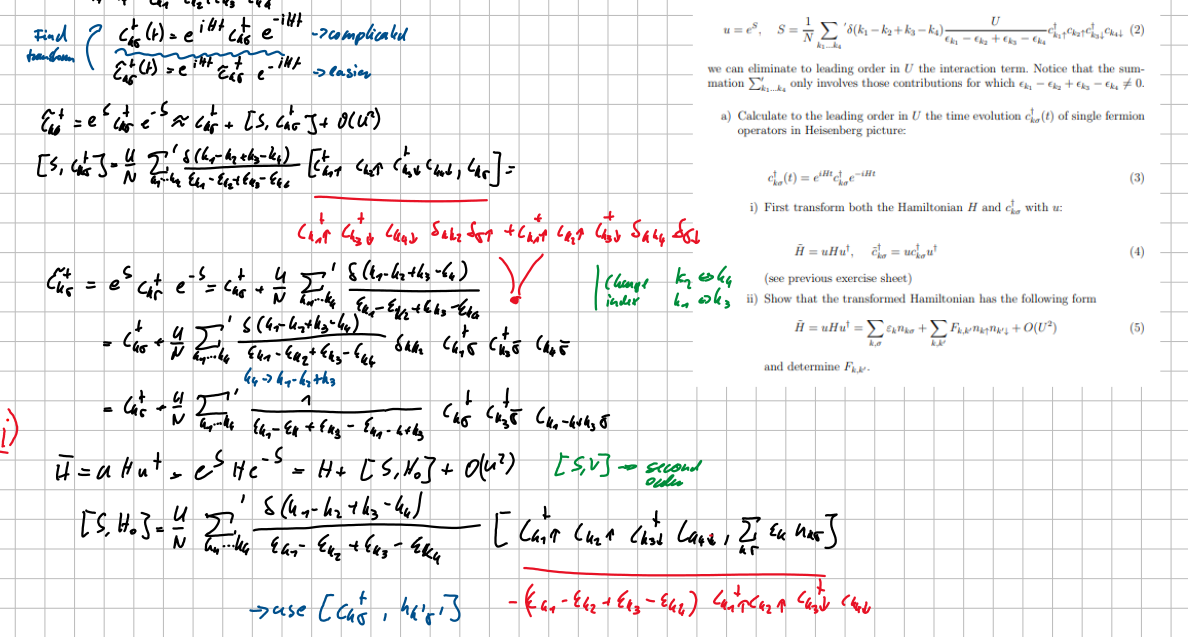
\includegraphics[width=0.85\textwidth]{math-manipulator-calculations/fkp_page_33.png}}
    
\end{frame}

\note[enumerate]{
    \item From the lecture "Theoretical Solid State Physics" (Theoretische Festkörperphysik), helt by Markus Heyl in WS 22/23
    \item Sheet 8, Problem 1: Schrieffer-Wolf transformation of the Hubbard Model
    \item Just written down steps done by someone else (Tutor/other pupil, often shared the terms to calculate them all, still time)
}

\begin{frame}
    \frametitle{Examples from the Practical Training}

    \begin{columns}
        \column{0.4\textwidth}
            \begin{itemize}
                \item Goal: produce time evolution of operator
                \item Uses calculation in Interaction Picture
                \item Workflow:
                \begin{itemize}
                    \item Inserting Definitions
                    \item Expanding
                    \item Ordering
                    \item Rewriting efficiently
                \end{itemize}
            \end{itemize}
            
        \column{0.4\textwidth}
            \makebox[\textwidth][c]{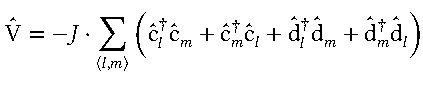
\includegraphics[page=1,width=.9\textwidth]{./main-content/paper/V_interaction_picture.pdf}}
            \vspace{0.3em}
            \makebox[\textwidth][c]{\includegraphics[page=2,width=.9\textwidth]{./main-content/paper/V_interaction_picture.pdf}}
            
    \end{columns}
\end{frame}

\note[enumerate]{
    \item Want to calculate the Time-Evolution of the operator V in the interaction Picture
    \item Basically comes down to inserting definitions (however already derived from MM)
    \item Distributing and re-ordering is a painful, time-intensive process
}
